\documentclass[a4,11pt,oneside]{article}
%\documentclass[a4,12pt]{practica}

\usepackage[english]{babel}
\usepackage{epsfig}
\usepackage{amssymb,listings,color,textcomp,marvosym,flafter,longtable,subfigure,amsfonts,rotating}
\usepackage[sumlimits]{amsmath}
\usepackage{verbatim}
\usepackage{latexsym}
\usepackage{multirow}
\usepackage{array,pstricks,listings}
\usepackage[a4paper,verbose, centering,reversemp]{geometry}
\usepackage[latin1]{inputenc} 
\usepackage{fancyhdr}
\usepackage{hhline}     % generates nicer table lines (without missing pixels) + more flexible
\usepackage[times]{quotchap} 
\usepackage[font={small},labelfont={bf},center]{caption}
% this package used to produce a different style of page numbering
%\usepackage{chappg}  
\usepackage{times}  
\usepackage{wrapfig}
\usepackage{floatflt}
% this package is used for colored text
\usepackage{xcolor}
% this package is used for intelligent spaces
\usepackage{xspace}
%\input{macros.tex}
\usepackage[calcwidth,newparttoc]{titlesec}
% use the titletoc package to change the toc
\usepackage{titletoc}
% this package is the natural frontend for pgf (a package for creating graphics in an inline manner).
\usepackage[round]{natbib}
\definecolor{chaptergray}{rgb}{0.85,0.85,0.85}
%\textwidth=15.5cm
%\textheight=23cm
\usepackage{enumerate}
\usepackage{pstricks,pstcol,pst-text,pst-node,pst-tree}
\usepackage{verbatim}
\usepackage[vlined,ruled,nederlands]{algorithm2e}
\usepackage{graphicx}
\usepackage{tabularx}
\usepackage{latexcad}
\usepackage{soul}
\usepackage{hyperref}
\usepackage{epstopdf}
\usepackage[framemethod=TikZ]{mdframed}
%\hypersetup{colorlinks=false}
\definecolor{silver}{rgb}{0.95,0.95,0.95}
\definecolor{chaptergray}{rgb}{0.95,0.95,0.95}
\font\sixly=lasy6 % does not re-load if already loaded, so no memory problem.

\usepackage{lmodern}
\usepackage[T1]{fontenc}

\mdfdefinestyle{warning}{%
    linecolor=white,
    align=center,
    roundcorner=3pt,
    innertopmargin=6pt,
    innerbottommargin=5pt,
    innerrightmargin=10pt,
    innerleftmargin=10pt,
    backgroundcolor=black!12,
    skipabove=0.4\baselineskip
}

%\input{macros.tex}

%\textwidth=15.5cm
%\textheight=23cm

\parskip=\medskipamount
%\parindent=0pt
\setcounter{secnumdepth}{3}
\newtheorem{mf}{MATLAB functie}[section]
\newtheorem{vb}{Voorbeeld}[section]

\newtheorem{voorbeelden}{Voorbeelden}[section]
\newtheorem{vraag}{Vraag}[section]
\newtheorem{opdracht}{Opdracht}[section]
\newtheorem{opdrachtE}{Assignment}[section]


\def\bea{\begin{eqnarray}}
\def\eea{\end{eqnarray}}
\def\beas{\begin{eqnarray*}}
\def\eeas{\end{eqnarray*}}

\def\pr{\mbox{Pr}}

\newtheorem{oefening}{Oefening}[section]
%\renewcommand\chaptername{Practicum}

\renewcommand{\algorithmcfname}{Algoritme}
%%%%%%%%%%%%%%%%%%%%%%%%%%%%%%%%%%%%%%%%%%%%%%%%%%%%%%%%%%%%%%%%%%%%%%
% document: page_layout_definition.tex
%
% last modified: $Id: page_layout_definition.tex,v 1.1 2005/11/18 11:49:23 bvolckae Exp $
%
% author: Filip De Turck, Stefaan Vanhastel, Bart Duysburgh, Brecht Vermeulen, Bruno Volckaert, Steven Van den Berghe
%%%%%%%%%%%%%%%%%%%%%%%%%%%%%%%%%%%%%%%%%%%%%%%%%%%%%%%%%%%%%%%%%%%%%%

%%%%%%%%%%%%%%%%%%%%%%%%%%%%%%%%%%%%%%%%%%%%%%%%%%%%%%%%%%%%%%%%%%%%%%

% basic dimensions when printing the small page %
% and by using the geometry package             %

% settings Filip en Stefaan
%\geometry{bottom=4.0cm,rmargin=4.25cm,body={12.5cm,19.5cm}} % 10pt op a4
%\geometry{marginpar=0.0cm,marginparsep=0.0cm,twosideshift=0.0cm}

% new settings (according book pim which was approved by the promotors) by Bart Duysburgh
%\geometry{bottom=5.34cm,rmargin=4.5cm,body={11.5cm,18.92cm}} % 10pt op a4
%\geometry{marginpar=0.0cm,marginparsep=0.0cm,twosideshift=0.0cm}
%body={16.5cm,24cm}
\geometry{bottom=2.5cm,rmargin=2.25cm,lmargin=2.5cm,top=2.6cm} % 10pt op a4
%\geometry{bottom=5.34cm,rmargin=4.5cm,body={11.5cm,18.92cm}} % 10pt op a4
\geometry{marginpar=2.5cm,marginparsep=0cm}

%\geometry{bottom=2.15cm,rmargin=2.5cm,body={14.14125cm,23.6cm}} % 12pt op a4

%\renewcommand{\headwidth}{17cm}                % Resetten van al de fancy settings.%
%\renewcommand{\headrulewidth}{0.4pt}      % Zet dit op 0.4pt voor een mooie lijn. geen lijn: 0pt
%\textwidth=15.5cm
%\textheight=23cm
%%%%%%%%%%%%%%%%%%%%%%%%%%%%%%%%%%%%%%%%
%\topmargin=0cm
%\headsep=.7cm
\setlength{\textwidth}{16.5cm}
%\setlength{\textheight}{24cm}
%\setlength{\topmargin}{0.0cm}
%\setlength{\oddsidemargin}{0.7cm}
%\setlength{\evensidemargin}{0.7cm}
%\setlength{\marginparwidth}{0pt}
%\setlength{\marginparsep}{0pt}


%%%%%%%%%%%%%%%%%%%%%%%%%%%%%%%%%%%%%%%

%\renewcommand{\topfraction}{0.8}

%%%%%%%%%%%%%%%%%%%%%%%%%%%%%%%%%%%%%%%

%%%%%%%%%%%%%%%%%%%%%%%%%%%%%%%%%%%%%%
%% change for subfigure
\renewcommand{\subfigcapskip}{0pt}
%%%%%%%%%%%%%%%%%%%%%%%%%%%%%%%%%%%%%%

%%%%%%%%%%%%%%%%%%%%%%%%%%%%%%%%%%%%%%%
% headings %

\fancypagestyle{plain}{
\fancyhf{}
\renewcommand{\headrulewidth}{0pt}
\renewcommand{\footrulewidth}{0pt}}

\pagestyle{fancy}
\fancyhf{} %clear all header and footer fields
%\addtolength{\headwidth}{\marginparsep}
%\addtolength{\headwidth}{\marginparwidth}

\renewcommand{\chaptermark}[1]{\markboth{\chaptername\ \thechapter. \ #1}{}}

%\renewcommand{\chaptermark}[1]{\markboth{#1}{}}
%\renewcommand{\sectionmark}[1]{\markright{\thesection\ #1}}

%\newcommand\fdtsvrightmarktmp{{\scshape\small Chapter }}
%\newcommand\fdtsvrightmark{{\scshape\small{Acknowledgment}}}
%\newcommand\fdtsvleftmark{{\scshape\small{Dankwoord}}}

%\newcommand\oddpageleftmark{}
%\newcommand\evenpagerightmark{}

%\fancyhead[LE,RO]{\itshape\bfseries\small\thepage}
%\fancyhead[HL]{\itshape\bfseries\small\leftmark}
%\fancyhead[RE]{\itshape\bfseries\small\rightmark}
%\fancyfoot[FC]{\bfseries\small\thepage}
%\fancyhead[LO]{\oddpageleftmark}
%\fancyhead[RE]{\evenpagerightmark}
%\fancyhead[HL]{\nouppercase{\leftmark}}
%\fancyfoot[C]{\itshape\bfseries\footnotesize \chaptername\ \thechapter}

%%%%%%%%%%%%%%%%%%%%%%%%%%%%%%%%%%%%%%%%%%%%%%%%%%%%


%%%%%%%%%%%%%%%%%%%%%%%%%%%%%%%%%%%%%%%%%%%%%%%%%%%%
% depth of numbering and depth of table of contents %

\setcounter{tocdepth}{3} % titels tot en met niveau subsubsection worden in table of contents opgenomen
\setcounter{secnumdepth}{3} % tot en met niveau subsubsection wordt er genummerd
%%%%%%%%%%%%%%%%%%%%%%%%%%%%%%%%%%%%%%%%%%%%%%%%%%%



%%%%%%%%%%%%%%%%%%%%%%%%%%%%%%%%%%%%%%%%%%%%%%%%%%%
%%%%% Definition for Big letter at the beginning of a paragraph %%
\def\PARstart#1#2{\begingroup\def\par{\endgraf\endgroup\lineskiplimit=0pt}
    \setbox2=\hbox{\uppercase{#2} }\newdimen\tmpht \tmpht \ht2
    \advance\tmpht by \baselineskip\font\hhuge=cmr10 at \tmpht
    \setbox1=\hbox{{\hhuge #1}}
    \count7=\tmpht \count8=\ht1\divide\count8 by 1000 \divide\count7 by\count8
    \tmpht=.001\tmpht\multiply\tmpht by \count7\font\hhuge=cmr10 at \tmpht
    \setbox1=\hbox{{\hhuge #1}} \noindent \hangindent1.05\wd1
    \hangafter=-2 {\hskip-\hangindent \lower1\ht1\hbox{\raise1.0\ht2\copy1}%
    \kern-0\wd1}\copy2\lineskiplimit=-1000pt}
%%%%%%%%%%%%%%%%%%%%%%%%%%%%%%%%%%%%


%%%%%%%%%%%%%%%%%%%%%%%%%%%%%%%%%%%%%%%%%%%%%%%%%%%%
%%% Nog een paar andere zaken  %%%%
%% om een cross-ref naar een voetnoot te kunnen maken definier ik \usefn %%
%\newcommand{\usefn}[1]{\mbox{\textsuperscript{\normalfont#1}}}
%
%\setlength{\captionindent}{1cm}
%\renewcommand{\captionfont}{\small \itshape \mdseries \rmfamily}
%\renewcommand{\subcapsize}{\footnotesize \itshape \mdseries \rmfamily}
%
%\AtBeginDocument{%
%%   \renewcommand{\figurename}{Fig.}%
%%   \renewcommand{\tablename}{TABLE}%
%   \renewcommand{\tablename}{Table}
%   \renewcommand{\bibname}{References}%
%}

%%%%%%%%%%%%%%%%%%%%%%%%%%%%%%%%%%%%%%%%%%%%%%%%%%%


\renewcommand{\baselinestretch}{1.2}
% space between two paragraphs should be larger than between two lines of text
\newcommand{\npar} {\par \vspace{2.3ex plus 0.3ex minus 0.3ex}} 
% no indentations
\setlength{\parindent}{0cm}
% makes all pages the height of the text on that page, and no extra vertical space is added
\raggedbottom
\renewcommand\chaptertitlename{PC-lab}


% define part label
\titleformat{\part}[display]{\flushright\bfseries\vspace{-10cm}} 
{\usefont{OT1}{pag}{b}{n}\fontsize{50}{54}\selectfont{PART~\thepart}} {0pt} {\vspace{0.5cm}\huge\usefont{OT1}{pag}{m}{n}\fontsize{25}{30}\selectfont\uppercase} [\thispagestyle{empty}\pagecolor{chaptergray}]
% define chapter label
\titleformat{\chapter}[display]{\flushright\vspace{-3cm}\pagecolor{white}}
{\usefont{OT1}{pag}{b}{n}\fontsize{34}{34}\selectfont {\chaptertitlename\quad\thechapter}}{10pt}{\usefont{OT1}{pag}{m}{n}\fontsize{22}{24}\selectfont}[{\thispagestyle{empty}\vspace{3cm}}]
% define section label
\titleformat{\section}[hang]{}
{\usefont{OT1}{pag}{b}{n}\fontsize{14}{16}\selectfont\thesection}{16pt}{\usefont{OT1}{pag}{b}{n}\fontsize{14}{16}\selectfont}[{}\vspace{0.25cm}]

\titleformat{\subsection}[hang]{}
{\usefont{OT1}{pag}{b}{n}\selectfont\thesubsection}{13pt}{\usefont{OT1}{pag}{b}{n}\selectfont}[{}\vspace{0.25cm}]
% define subsubsection label
\titleformat{\subsubsection}[hang]{\sffamily}
{\usefont{OT1}{pag}{m}{n}\fontsize{11}{12}\selectfont\thesubsubsection}{13pt}{\usefont{OT1}{pag}{m}{n}\fontsize{11}{12}\selectfont}[{}\vspace{0.05cm}]
% define paragraph label
\titleformat{\paragraph}[runin]{\sffamily}
{\usefont{OT1}{pag}{b}{n}\selectfont\theparagraph}{}{}[{}]

% define the headers and the footers
\renewcommand{\chaptermark}[1]%
 {\markboth{ \MakeUppercase{CHAPTER~\thechapter \mdseries{~~~#1}}}{}}
\renewcommand{\sectionmark}[1]%
 {\markright{\fontsize{10}{12} \selectfont\MakeUppercase{\thepart.\thesection \mdseries{~~~#1}}}}
\renewcommand{\headrulewidth}{0.15pt}
\renewcommand{\footrulewidth}{0pt}
\newcommand{\helv}{%
\fontfamily{phv}\fontseries{b}\fontsize{8}{10}\selectfont}
\fancyhf{}
\fancyhf[HR]{\helv \fontsize{10}{12} \selectfont \thepage}
\fancyhf[HL]{\helv \fontsize{10}{12} \selectfont \rightmark}
%\fancyhf[HL]{\helv \rightmark}
%\fancyhead[RE]{\helv \rightmark}


%\texttt{}
\hyphenation{bij-ge-volg ge-wij-zigd toe-pas-sing toe-pas-sing-en
lid-maat-schaps-func-ties ver-ge-lijk-ing-en va-ria-be-le
pa-ra-me-ter-s pa-ra-me-ter in-gangs-var-ia-be-le
uit-gangs-var-ia-be-le glo-ba-le sym-bo-li-sche be-schik-king
ver-wer-ven zoek-me-tho-den pro-ba-bi-li-teit ge-ne-ra-tie
ver-dui-de-lij-ken de-co-de-ring af-wij-king-en drie-hoe-ki-ge
tra-pe-zo clus-ter-al-go-rit-mes uit-ein-de-lijke tracht fi-gu-ren ge-lijk-aardig mo-ge-lijke ge-lijk-aardige op-ti-ma-li-sa-tie-pro-ble-men pro-bleem-spe-ci-fie-ke}

\lstset{language=R,commentstyle=, framexleftmargin=5mm,belowcaptionskip=5mm, frame=single,basicstyle={\ttfamily\small}, stringstyle=\small,commentstyle=\textcolor[rgb]{0.53,0.53,0.53}, backgroundcolor=\color[rgb]{0.93,0.93,0.93},showspaces=false,framexleftmargin=-2pt,showstringspaces=false,upquote=true}

\begin{document}
%\frontmatter
\renewcommand{\algorithmcfname}{Algorithm}
\pagestyle{empty}


\begin{titlepage}
	\begin{center}
		%{\rugfnt A}\\[.3cm]
		{\Large\bf GHENT UNIVERSITY}\\[.5cm]
		{\Large Faculty of Bioscience Engineering}\\[.5cm]
		{\Large Department of Mathematical Modelling, Statistics and Bioinformatics}\\[.5cm]
		\hrule{\ }\\[.4cm]
	
		\vspace{4cm}
\begin{mdframed}[style=warning]
		\vspace{1cm}
\centering
		{{\huge \bf Machine Learning for Image Processing}}\\[1cm]
		{\LARGE Predictive Modelling - Project 1}
		\vspace{1cm}
\end{mdframed}
		\vspace{3cm}


	\end{center}
	
	\begin{center}
		{\large \bf ir. Jim Clauwaert\\[.2cm]
		\large \bf ir. Marlies Volckaert\\[.2cm]
		\large \bf ir. Michael Ghijs\\[.2cm]
%		\\[.1cm]
		}%\\
		
		\vfill
%		Master in Bioscience Engineering\hfill
		Academic year 2016--2017\\[.3cm]
		\hrule \vspace{.3cm}
%		\noindent {\tt http://www.kermit.ugent.be}
		% \noindent {\tt http://biomath.UGent.be/\~{ }kcmaes}
	\end{center}
\end{titlepage}





%%%  --> BEGIN OLD frontpage

%\begin{titlepage}
%\begin{center}
%%{\rugfnt A}\\[.3cm]
%{\Large\bf GHENT UNIVERSITY}\\[.5cm]
%{\large Faculty of Bioscience engineering}\\[.4cm]
%\hrule{\ }\\[.4cm]
%{\large Department of Mathematical Modeling, Statistics and Bioinformatics}
%
%\vspace{3cm} {\Huge \bf Machine Learning:\\[1cm]
%PC-labs}
%\end{center}
%
%\begin{center}
%\vspace{2cm} {\Large \bf Prof.\ Dr.\ Bernard DE BAETS\\[.1cm]
%Dr. Willem WAEGEMAN\\[.25cm]
%Ir. Jan VERWAEREN}
%\vspace{2cm}
%\begin{center}
%\includegraphics[width=3.5cm]{figures/Kermit.eps}
%\end{center}
%\vfill
%Course notes for\\[.3cm]
%``Machine Learning''\\[.3cm]
%Master in Bioscience engineering\\[.3cm]
%Academic year 2012--2013\\[.3cm]
%\hrule
%\vspace{.3cm}
%
%\noindent {\small\tt http://www.kermit.ugent.be}
%\end{center}
%%\end{document}
%\newpage
%~ 
%\end{titlepage}

%%%  --> END OLD frontpage






%\newpage
%\pagestyle{empty}
%~
%\newpage
%\setcounter{page}{1}
%\pagestyle{fancy}
%\tableofcontents
%\newpage
%\thispagestyle{empty}
~
%\mainmatter
%\setcounter{page}{-1}
%\part[Introduction To Machine Learning]{Introduction To\\ Machine Learning}

%\pagestyle{empty}
%\newpage
%~
%\newpage
%\pagestyle{fancy}
%\setcounter{page}{1}

%\parindent=0cm
%\setcounter{chapter}{7}
%\documentclass{article}
%\usepackage{graphicx}
%\usepackage{tabularx}
%\usepackage [dutch] {babel}
%\usepackage[vlined,ruled,algo2e]{algorithm2e}

\newcommand{\xvect}{\mathbf{x}} 
%\chapter[Scientific programming for Machine Learning]{Scientific programming for\\ Machine Learning}
%\begin{document}
%\chapter{\emph{Hill Climbing} en \emph{Simulated Annealing}}\label{pract: HC}
\section{From cable transmission to far beyond: \\ applications and evolution of image processing \label{sec:evolution}}
Early digital image processing began in the early 1920s with the Bartlane cable picture transmission system that was used to transmit newspaper images across the Atlantic (Figure~\ref{fig:bartlane}). The images were coded and sent by telegraph. It took about three hours to send an image and the first systems supported only five grey levels. Along with the first satellite images in the beginning of the 1960s, image processing further emerged. Although computers were slow at the time and their processing capacity very limited, image processing was used for weather forecasting, military purposes, land use detection etc. 

\begin{figure}[h]
	\centering
	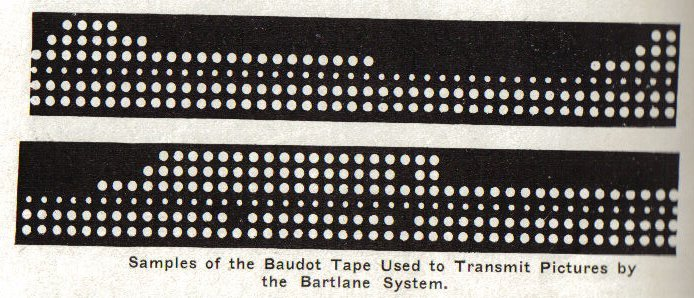
\includegraphics[width=0.5\textwidth]{../figures/Bartlane}
	\caption{Code used by the Bartlane transmitter to transport newspaper images.
		\label{fig:bartlane}}
\end{figure}

As the computers evolved, so did digital image processing and algorithms became more and more complex: today, automated image recognition is omnipresent. Think about Google images, criminal detection, fingerprint scans at the airports, smart radars, detection of cancer cells etc. 


Computer vision, or machine vision, means the use of digital processing and intelligent algorithms to interpret meaning from images or video. Machine vision definitely is a hot item: currently self-driven cars and buses are in full development and the first prototypes are being tested which make use of 3D-real time computer vision. 
\begin{figure}[h]
	\centering
	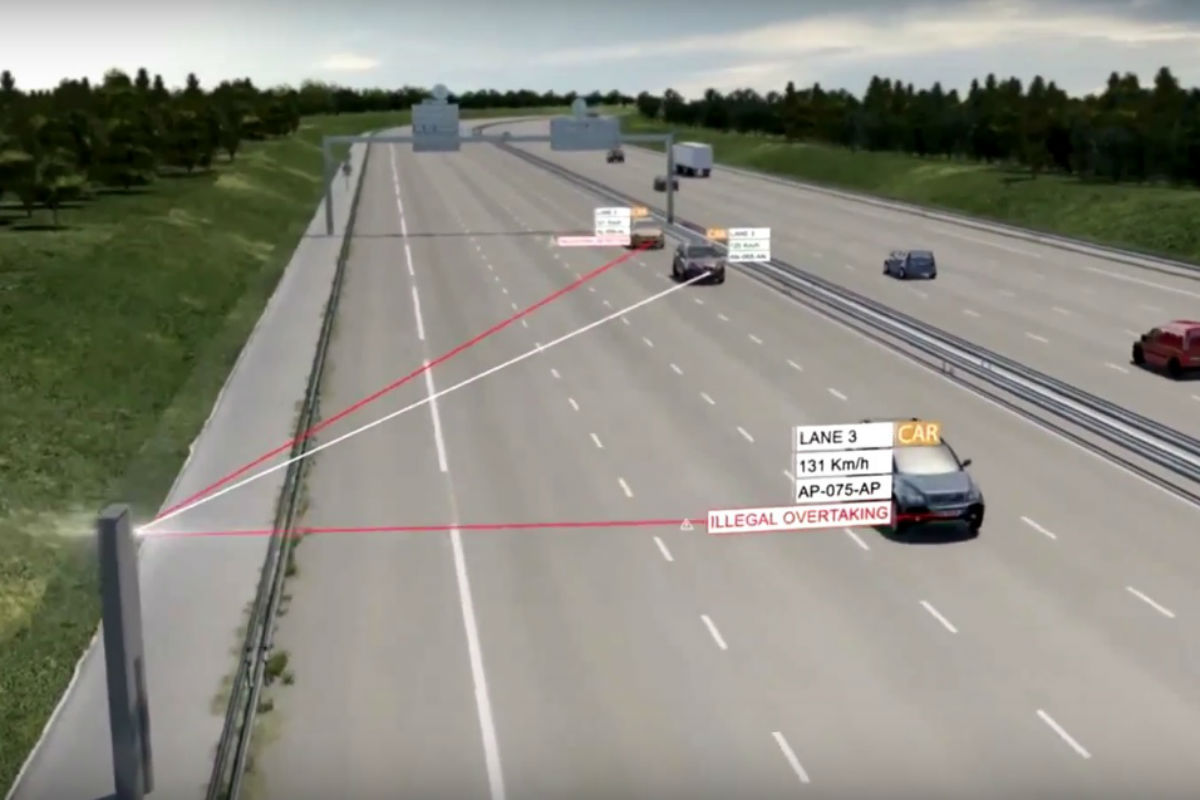
\includegraphics[width=0.5\textwidth]{../figures/Mesta-Fusion}
	\label{fig:flitspaal}
	\caption{The Mesta Fusion traffic radar is coming to our roads and is already operational in some European countries. It uses machine vision technologies to track 32 cars at a time, for license plate recognition among others.}
\end{figure}

Today a major transformation is underway. Due to the emergence of very powerful, low-cost, and energy-efficient processors, it has become possible to incorporate practical computer vision capabilities into embedded systems, mobile devices, PCs, and the cloud. Over the next few years, there will be a rapid proliferation of embedded vision technology into many kinds of systems. Take `Project Tango' from Google as an example: it uses (small) smartphone cameras to picture the 3D-structure of the space in which a person is situated. Just imagine this technology in real-time games!

\section{From human vision to computer vision: principles and mechanisms \label{sec:mechanisms}}
When a 3-year child looks at an image, it can already detect what it sees: an airplane taking off, a cat sitting on a couch, a tree in a park, etc. That child is already an expert in making sense to what it sees. Our most advanced technological systems still struggle with this task.
The human eye is a sensor that catches light on the retina, the optic nerve transports the impulses to the brains and there the magic happens: sophisticated neural networks analyze the images and give meaning to it. Vision begins at the eyes, but it truly takes place in the brains. 
Computer vision is based on the same principles as human vision. Cameras register the incoming light as digital numbers in a 2D (or 3D) array. Besides the intensity of the incoming light, pixels do not have a meaning, they do not say what is in the picture. In order to understand a picture, a computer needs to apply the entire Image Processing Chain, see Figure~\ref{fig:imProChain}:

\begin{figure}[h!]
	\centering
	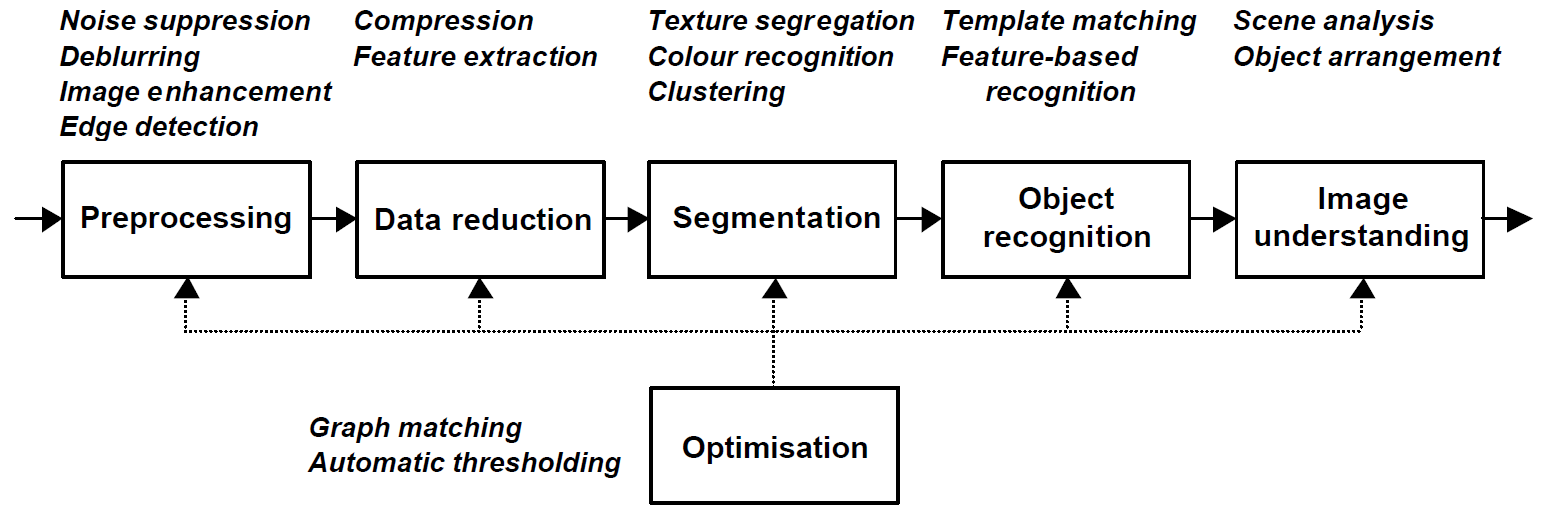
\includegraphics[width=\textwidth]{../figures/imageProcessingChain}
	\caption{Classical image processing chain.  \citep{Egmont-Petersen2002} 
		\label{fig:imProChain}}
\end{figure}

\begin{enumerate}
	\item \textbf{Pre-processing}:
	Images can contain a lot of noise and could therefore difficult to interpret. Think for example of Rayleigh scattering in satellite images which result in a very low contrast, or photographs that look blurry because they were taking while moving. Pre-processing consists of operations that modify the original image in order to make it more interpretable: e.g. noise reduction and contrast enhancement.
	
	
	\item \textbf{Data reduction}:
Hyperspectral satellites process incoming light at more than thousand different spectral bands. The information coming from this images is enormous and not all information is equally useful. Only the bands which carry the most information for a specific application are selected. If we take a look to a single image, features (entropy, contrast, heterogeneity etc.)  can be extracted by means of moving windows. The number of features extracted is generally smaller than the number of pixels in the input window. 

\item \textbf{Segmentation}:
The partitioning of the image into regions with similar characteristics (spectral, textural features). 

\item \textbf{Object detection and recognition}:
Once the image is divided into segments, these segments can be classified. The position, orientation and scale of objects (possibly consisting of multiple segments) can be determined. 

\item \textbf{Image understanding}:
Deriving high level knowledge, semantic data, from an image. E.g. there is a cat on the table (and the cat is hungry trying to steal pork ribs).

\end{enumerate}

\section{Copying the brain: Convolutional Neural Networks \label{sec:cnn}}
\textit{Neural networks} are a computational approach inspired by the structure of the brain, as the resulting models are large collections of interconnected neurons, connecting inputs to a prediction (Figure~\ref{fig:ann}). They are used in various image processing applications, e.g. to optimise different steps in the image processing chain. \textit{Convolutional neural networks} are a more recent strategy in artificial intelligence, using neural networks to copy the abilities of a three-year-old child in image recognition.
\begin{figure}[h!]
	\centering
	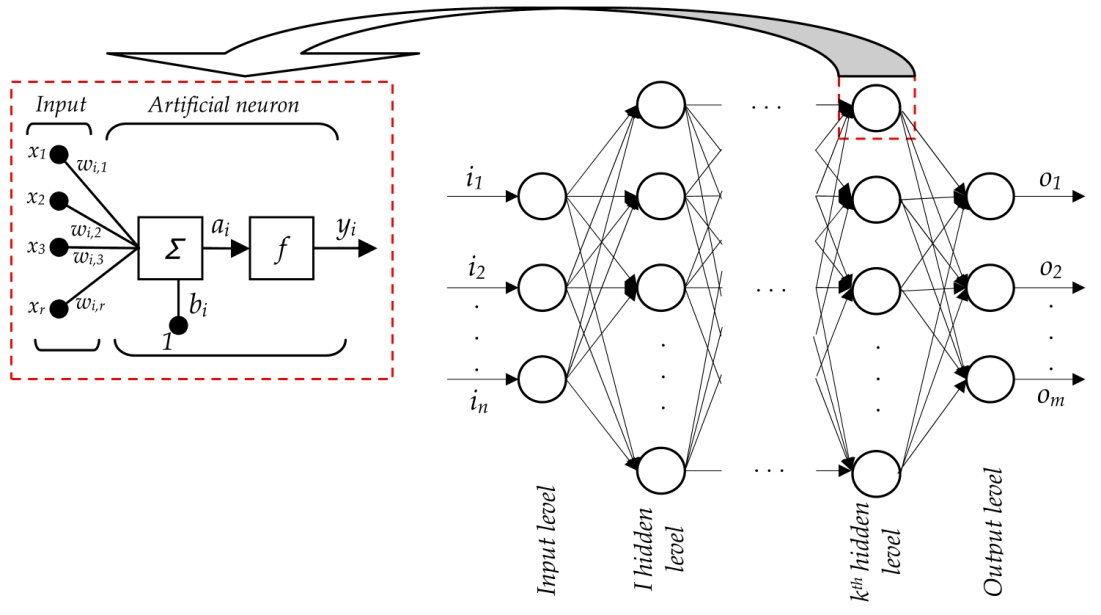
\includegraphics[width=\textwidth]{../figures/ann_struct}
	\caption{Neural network.
		\label{fig:ann}}
\end{figure}

\subsection{The basics: Neural networks \label{subsec:neural}}
Neural networks process a number of inputs with a set of artificial \textit{neurons} in order to generate its model output, i.e. a prediction. These neurons individually can take in multiple inputs and process them in two steps to formulate an output: aggregation of the inputs and consecutively linking them to the output with an activation function. The output is a certain value representing the (amount of) activation of the neuron. 


In the \textit{aggregation step}, \textit{weights} $\textbf{w}$ are given to the different inputs of the neuron, indicating their influence on the neuron\textquoteright s output. The weights are multiplied with the input values and summed, calling for a \textit{threshold} or \textit{bias} $\textbf{b}$, to tell whether or not the aggregated value leads to activation of the neuron. If $\sum{\textbf{wx}} > \textbf{b}$, the neuron is activated, otherwise it is not; this can be seen as a step function between 0 and 1.


This would be the basic construction for the neuron, yet the step function can prove cumbersome for the training of the neural network. Therefore, the aggregated value and bias themselves are linked to the actual neuron output by an \textit{activation function}. The commonly used activation functions are presented in Section~\ref{subsec:activation}. 


The output of neurons can then be connected to other neurons. The structure of a neural network usually consists of layers of neurons, the first one processing the inputs and passing on their outputs to the second layer, while the last layer generates the prediction (see Figure~\ref{fig:ann}). This is detailed in Section~\ref{subsubsec:archi}.


\subsubsection{Commonly used activation functions \label{subsec:activation}}
A historically used function, attractive because of its similarity to the biological neuron, is the \textit{sigmoid function}, presented in FIGUUR+VGN. It `squashes\textquoteright  a real input into the range between 0 and 1. Neural network applications have moved on from this function however. As the tails of the function have a very low slope - which is used in training the neural network (see section later on) -  the sigmoid function can cause that the neuron goes unnoticed during training. Next to this major drawback, a minor inconvenience of the sigmoid function is that the output is always positive, of which the consequences will be explained in Section BackpropagationREF.


A similar activation function is \textit{Tanh} FIGUUR+VGN, which has a similar shape as the sigmoid function and mitigates the aforementioned issue by squashing its input between -1 and 1, allowing for negative output values. 


Another function, the \textit{Rectified Linear Unit} or \textit{ReLU} FIGUUR+VGN, basically thresholds the input at 0. They were found to greatly accelerate training of the neural network (\cite{Krizhevsky2012}), said to be due to its linear form. Compared to the first two activation functions, ReLUs are easy to implement and to compute. Despite their popularity, ReLUs have the major drawback that they can \textquoteleft die\textquoteright  during training, which means that they do not activate on any datapoint anymore. This can occur in the case that a large gradient flows through the neuron, which could lead to the weights being updated in a way that no inputs can still activate the neuron FIGUUR. At high learning rates the risk of this \textquoteleft death\textquoteright  is high and large part of the network can turn out to be deactivated.


To accommodate for the ReLU \textquoteleft neuron death\textquoteright  issue, \textit{Leaky ReLUs} FIGUUR+VGN have a small constant negative slope at levels below 0.


Last but not least is the \textit{softmax} function VGN, which is distinct from the aforementioned activation function because it relates the output of a single neuron to the outputs of all neurons in the layer. By dividing by the sum of all these outputs, the output of a single softmax neuron is always between 0 and 1, and the sum of all activations is 1. 
%Finally, there are also activation functions that are out-of-the-box, such as the Maxout neuron. This activation function takes the maximum of the output of two different activation functions computed on the input. While this can solve issues related to the aforementioned functions, the amount of parameters in the model is increased.

\subsubsection{Network architecture \label{subsubsec:archi}}
Neural networks are usually built out of \textit{layers of neuron}s, in which a layer can be seen as a group of neurons where information can only be propagated to the next layer, thus without having connections between neurons in the same layer (visible in Figure~\ref{fig:ann}). These are \textit{feedforward neural networks}, yet other classes of neural networks also exist, such as recurrent neural networks, which do allow self loops on neurons.


%The \textit{size} of a neural network is usually expressed in the number of neurons or, even more commonly, as the number of parameters in the network. For example, the network in FIgure has this amount of parameters. Convolutional neural networks nowadays contain on orders of 100 million parameters and are usually made up of approximately 10 to 20 layers.
% % %%EXAMPLE

\subsubsection{Training a neural network \label{subsubsec:training}}
Training a neural network means optimising its parameter values so that its prediction is as close to the real data as possible. The difference between the predicted and real values is represented by a \textit{loss function}. This function can take the form of a quadratic function, such as the SSE, yet this could result in a \textit{learning slowdown problem} due to the nature of the neurons. In a multi-class classification problem, which is common in image processing, taking for example the sigmoid neuron, one can see that in the tails of the output the slope is very low. Therefore, for these problems, a specific loss function has been developed, called \textit{cross-entropy} VGN. This loss function takes into account the structure of the activation function. Namely, when the cross-entropy loss function is derived to the network parameters, it is proven that this derivative is dependent on the difference between the neuron output and the real data. Ergo, the larger this difference, the faster the weights are changed to find a better optimum.


Other loss functions can still be applied in cases where these are feasible. Also, in the case of a softmax neuron layer, the learning slowdown problem is already intrinsically addressed.


For \textit{minimising} the loss function, the slope or \textit{gradient} of the loss function, in function of the model output, is the starting point. Following the gradient towards a minimum is therefore the mechanism in the most used optimisation algorithm for neural networks, namely \textit{gradient descent}. Another reason for its popularity though, is that the gradient can also be found for the loss function in function of the values of the model parameters. This technique is called backpropagation and applied the chain rule of function derivatives. FIGUUR? With this gradient, a set of optimal values for the parameters can immediately be explored for using gradient descent, a feature that allows for a much faster neural network training than by using other gradients.

\subsection{Convolutional neural networks \label{subsec:cnn}}
The concept of convolutional neural networks is illustrated by applying it to an image of a wild boar (Figure~Figuur Marlies). The image consist of a 2D-array of pixels with a certain gray-level intensity. The image is split into pieces and for each patch, $A$ will compute features. In fact, $A$ is a group of neurons in parallel. They get all the same inputs pixel values and compute different features (contrast, entropy, homogeneity among others). If the patch contains e.g. a \textquoteleft pyjama\textquoteright  (other word for a wild baby boar), this will result in a specific vertical texture: high frequency (repetition of very bright pixels, followed by very dark pixels). In the snow regions on the other hand, contrast will be very low.

The neurons ($A$) in this layer are all fully connected ($F$). The convolution step can be repeated several times by putting a collection of  $A$\textquoteright  s as input in a second neuron layer, etc.
 
To reduce data, convolutional layers are often interweaved with pooling layers. Maximum pooling takes the maximum of features over a small block of input neurons. For a given patch of pixels the output of the maximum pooling step tells us if their is a high frequency, but not exactly where the high frequency is located. Maximum pooling has the benefit that higher layers can work on larger sections of data and that the output is made invariant to very small transformations of the data.
The output of the pooling layer is then used as input for another fully connected convolution layer and fed into the final neural network that is able to predict whether or not wild boar babies are present in the image. 


The entire classical image processing chain is integrated into this convolutional neural network. The separate steps are implicitly present at the different stages. Images are deliberately blurred to be used as input for these models so that the algorithm is capable of detecting objects regardless of any image artifacts. This is a major stumbling stone: machine learning only works when you have -a lot of- data to train the model. 

HIER MOET NOG INFO KOMEN OVER ARCHITECTUUR, OPTIMALISATIE E.D.

DAARNA LINKEN MET VOLGENDE SECTIE

\section{Neural Network Libraries \label{sec:libraries}}
A variety of libraries are available for image analysis using neural networks. For Python, the programming language chosen to use in this report, multiple options exist. Tensorflow, an open source library released by Google Brain can be considered the most popular choice at this moment. Since its release in November 2015, the project has enjoyed over 11.394 commits from over 500 different contributors on GitHub \url{https://github.com/tensorflow/tensorflow} . The library is used across the majority of services offered by Google. The library uses Python for its API while counting on the C++ programming language for under the hood calculations. 


TFlearn is a library built on top of TensorFLow to provide a higher-level API, offering the user more intuitive and easy-to-use functionality for the creation and implementation of (deep) neural networks. Although first released in late March 2016, it has received high popularity with contributions from over 60 developers \url{https://github.com/tflearn/tflearn}.
 
\subsection{Image datasets \label{subsec:imdata}}
The validation of deep neural networks for Image processing techniques are highly partitioned into the specific function of the model and the type of data it is optimized for. As trained models are highly correlated to those parameters their performance is dependent on the dataset it is validated with. A model can be created to recognize a single object for its input, but can also be engineered to recognize different objects from a scene, and partition it accordingly. Other models are trained to recognize and extract faces from moving pictures (video) or are specialized in the recognition of a single function. (e.g. reading the house number from street view pictures). 


As the quality of a model is highly dependent upon the function it performs, a variety of high quality datasets are used upon which optimization of a model is often performed. Examples of used image datasets are MNIST, CIFAR-10, CIFAR-100 and The Street View House Numbers dataset (SVHN). The MNIST database is a collection 70.000 handwritten digits centered on a grayscale 28 by 28 pixel image.  It has long been the standard dataset for the comparison of methods for a wide range of machine learning techniques. A compendium listing high accuracy models over a broad range of machine learning techniques is featured on the MNIST website (\url{http://yann.lecun.com/exdb/mnist/}). Techniques include SVM, Non-Linear Classifier, K-Nearest Neighbors and Neural Networks. 

CIFAR-10 and CIFAR-100 are a collection of coloured (three layers) 32 by 32 pixel images featuring a centered object.  Both feature 60.000 images where CIFAR-10 features ten different labels and CIFAR-100 a hundred. The SVHN dataset furthermore features a set of 73257 images of one or more digits featured in a 32 by 32 image. Unlike training on the MNIST dataset, models require the ability to extract and recognize multiple digits on one image. The documentation on new techniques adapted for training a model one one of these datasets with the resulting accuracy and error can be found here:   (\url{http://rodrigob.github.io/are_we_there_yet/build/classification_datasets_results.html}).


\subsection{Practical use-case \label{subsec:case}}
In this practical use-case we will aim to train a model to recognize humans. As no supercomputers were available for this work, tiny images were used to limit data processing requirements. For this, the CIFAR-100 dataset was used as a base and further enriched with images from humans. Only two possible predictions are executed by the model, being either \textquoteleft human\textquoteright  or \textquoteleft not human\textquoteright . This further limits the requirements of the processor as highly accurate training is achieved in a faster and more simple way than training to recognize a high amount of labels. 
The CIFAR-100 datasets has both coarse and fine labels. There are one hundred fine labels dividing the dataset. For every five fine labels there is a superclass that encompasses all five classes: the coarse label. Specifically, CIFAR-100 has  the coarse label \textquoteleft human\textquoteright  which consists of the five classes \textquoteleft baby\textquoteright , \textquoteleft boy\textquoteright , \textquoteleft girl\textquoteright , \textquoteleft man\textquoteright , \textquoteleft woman\textquoteright . 
After importing the required packages, we change the labels for human pictures to be class 1 and labels that are not pictures from humans to be class 2:

\begin{lstlisting}[caption= welke caption?, label=humanlabels]
te_labels = np.array([0 if u!= 14 else 1 for u in te_clabels100])
tr_labels = np.array([0 if u!= 14 else 1 for u in tr_clabels100])

\end{lstlisting}

Since our dataset contains mainly pictures of not humans, we wish to increase our pool of pictures of humans. For this, we enriched the CIFAR-100 dataset with the Frames Labeled In Cinema (FLIC) (\url{http://bensapp.github.io/flic-dataset.html})  dataset and images from the WIDER FACE dataset (\url{http://mmlab.ie.cuhk.edu.hk/projects/WIDERFace/}). We changed all the labels for these datasets to \textquoteleft 1\textquoteright . An overview of all the used data is given in Table~\ref{tab:data}.

\begin{table}[h]
	\centering
	\caption{Data used to train and test the model. \label{tab:data}}
	\begin{tabular}{|l|llll}
		\hline
		\textbf{() = \% human} & \multicolumn{1}{l|}{\textbf{CIFAR100}} & \multicolumn{1}{l|}{\textbf{FLIC}} & \multicolumn{1}{l|}{\textbf{LFW}} & \multicolumn{1}{l|}{\textbf{Total}} \\ \hline
		\textbf{Train}         & 50000 (5\%)                            & 3528 (100\%)                       & 11233 (100\%)                     & 64761 (26.65\%)                     \\ \cline{1-1}
		\textbf{Test}          & 10000 (5\%)                            & 1026 (100\%)                       & 2000 (100\%)                      & 13026 (27.00\%)                     \\ \cline{1-1}
		\textbf{Total}         & 60000 (5\%)                            & 4554 (100\%)                       & 13233 (100\%)                     & 77.787 (26.72\%)                    \\ \cline{1-1}
	\end{tabular}
\end{table}



After obtaining and processing our input data, shown in Listing X2, the main function is executed. For this, we use the example function from TFLearn for creating a model using CIFAR-10 (\url{https://github.com/tflearn/tflearn/blob/master/examples/images/convnet_cifar10.py}). As our resources are limited, and our model is only meant to be used as a proof of concept, only full iterations (epochs) over the whole dataset are done while executing the code.
\subsection{Gradient descent variants \label{subsec:gradient}}
Image recognition through the use of deep neural networks is still in its early phase as a study domain, where lots of new techniques are tried out on models to understand its interaction. Techniques in determining the optimal parameters are typically determined through the use of minimizing cross- entropy. Gradient descent, the determination of the gradient of  a specific set of parameters can be used to achieve the goal of finding minima. Multiple techniques have been created that are identified through the way the gradient of a set of parameters is used to determine a new set of parameters. Where first we discussed ways to obtain a gradient, an elaboration is now given on different ways of using the obtained information.
\subsubsection{Momentum \label{subsubsec:momentum}}
Momentum helps to accelerate finding a minimum as it takes into account the gradient of the previous step. Doing this, it tries to dampen the oscillation of the different gradients. 
$$v_t = \gamma v_{t-1} + \eta \nabla_\theta J( \theta)$$
$$ \theta = \theta - v_t $$
\subsubsection{Nesterov accelerated gradient \label{subsubsec:nesterov}}
The Nesterov accelerated gradient (NAG) takes into account the possibility that the momentum algorithm can adjust the parameters too much, missing a minimum and possibly ending up with a parameter set that leads to a different minimum. Instead of predicting the gradient of the loss function for the current step of parameters, NAG takes the gradient of the parameter set that has already been adjusted by the momentum of the previous iteration, as displayed in Figure~\ref{fig:nag}.

\begin{figure}[h!]
	\centering
	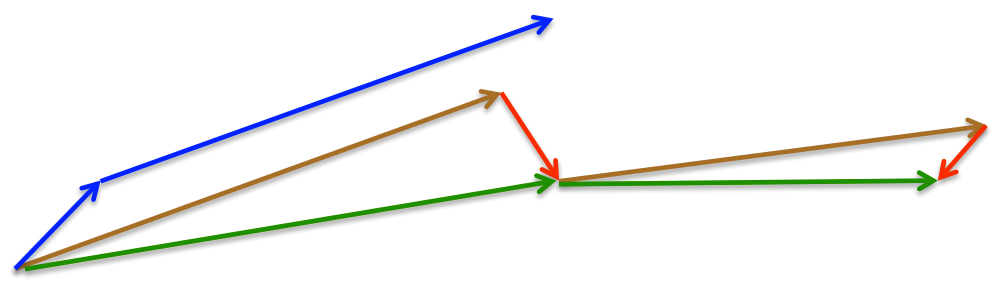
\includegraphics[width=0.6\textwidth]{../figures/nag}
	\caption{Depiction of the Nesterov accelerated gradient. Blue vector indicate the change of the parameterset of the momentum algorithm. The small vector represents the current gradient while the large vector signifies the updated accumulated gradient. The red vector indicates the gradient of the parameter set after adjustment by the accumulated gradient of the momentum (brown vector), resulting in an adjusted set of parameters (green vector).
		\label{fig:nag}}
\end{figure}

$$v_t = \gamma v_{t-1} + \eta \nabla_\theta J( \theta - \gamma v_{t-1})$$
$$ \theta = \theta - v_t $$

\subsubsection{Adagrad, Adadelta and Adam \label{subsubsec:aaa}}
Adagrad, Adadelta and Adam are a set of techniques implemented to adapt the learning rate to the frequency for which a parameter is updated. Specifically, the learning rate of more frequent parameters is dampened over time, while parameters linked to sparse data are not affected. Adagrad was a first implementation of this principle for which the learning rate of the respective parameters diminishes according to the sum of squares of the gradients with respect to $\theta{i}$. Adadelta is an adjustment to  Adagrad dealing with an monotonically decreasing learning rate, using a decaying sum of squares to prevent the parameter to become too big. Adam, the latest and most used adjustment of the group keeps track of both the average of past gradients and squared gradients, having proven to be an even better technique in reaching the minimum efficiently.





$$ g_{t, i} = \nabla_\theta J( \theta_i ) $$


$$ \theta_{t+1, i} = \theta_{t, i} - \dfrac{\eta}{\sqrt{G_{t, ii} + \epsilon}} \cdot \nabla_\theta J( \theta_i )  $$


where:
$$G_{t} \in \mathbb{R}^{d \times d}$$

%When opening R (on a Windows system), the user automatically arrives at the R console, which is based on a question-and-answer model. When the user enters a new instruction and presses enter, the program performs the necessary actions and prints the result to the same window. Whenever R is ready to receive new input, it will print out its prompt `$>$'. To give a first impression of how R works, create a new data vector $a=(1,5,3,4,8,5,8,1,3)$ by typing the following instruction into the command line
%
%%\begin{lstlisting}[caption=SimpleArrayJob.sh,label=simplearrayjob]
%\begin{lstlisting}[caption=createVector.R,label=createVector]
%a<-c(1,5,3,4,8,5,8,1,3)
%\end{lstlisting}
%
%Alternatively, we can feed this expression to the console  by: (1) type it into a script file (from the menu bar select \texttt{File > New Script}) and (2) execute this script (select the lines you want to run and press \texttt{crtl + r}). We advocate the use of this kind of scripts since they allow you to store and reuse code fragments more efficiently.
%
%To get a feeling of the basic operations, try to execute and understand the following instructions
%
%\begin{lstlisting}[caption=manipulateVector.R,label=manipulateVector]
%a[3] # accessing elements of a vector
%a[2:6]
%a[a>3]
%a[-1]
%
%b1<-a[c(-1,-2)] # creating new vectors (note the assignment operator <-)
%b2<-rep(2,7)
%b3<-seq(1,4,0.5)
%b4<-1:7
%
%b5<-(b3-(b1+b2)/b4)^2  # basic mathematical operations on vectors, note
%# that all operations are element-by-element (it is advisable only to 
%# use vectors of equal length)
%\end{lstlisting}
%
%From the examples given above, it is clear that variables do not have to be declared by the user, since R does this automatically. The vector operations described above are quite simple and intuitive, note that understanding how they work is essential to be able to work with R.
%
%\section{Important data structures}
%In addition to vectors, several other types of data structures (generally called objects) are defined in R such as arrays, matrices, lists and functions.
%\subsection{Functions}
%The R language allows the user to create objects of the type function. These are true R functions that are stored in a special internal form and may be
%used in further expressions and so on. In the process, the language gains enormously in power,
%convenience and elegance, and learning to write useful functions is one of the main ways to make
%your use of R comfortable and productive. A function is defined by an assignment of the form
%\begin{center}
%\texttt{name <- function(arg1, arg2, ...) \{ expression \}}
%\end{center}
%This assignment instruction can be typed into a script and executed, as any other instruction. Its use is illustrated in the following example
%\newpage
%\begin{lstlisting}[caption=functionSyntax.R,label=functionSyntax]
%myMean<-function(x, y)
%{
% # calculate the mean of two vectors
% temp<-(x+y)/2
% return(temp) # the return statement causes the function to terminate
% # and return the argument (temp) as a new object 
%}
%
%#using myMean
%b5<-myMean(b1,b2)
%b5<-myMean(y=b2,x=b1) # equivalent instruction
%\end{lstlisting}
%R has been designed as a statistical language, for this reason, a lot of (mathematical) functions have been incorporated by the developers. Most of them have intuitive names and can be used in the same way as user-defined functions. Some examples of functions that operate on vectors are \texttt{mean( )}, \texttt{sum( )}, \texttt{length( )}, \texttt{min( )}. Most of these functions are accompanied by an extensive manual page, which can be accessed through the instruction 
%\begin{center}
%\texttt{help( nameOfFunction )}
%\end{center}
%\subsection{Arrays and matrices}
%Arrays are multi-dimensional generalizations of vectors. In fact,
%they are vectors that can be indexed by two or more indices and will be printed in special
%ways. As for vectors, operations on arrays are typically performed element-by element. A matrix is simply a 2-dimensional array. Moreover, matrices allow matrix multiplication, as illustrated in the following example.
%
%\begin{lstlisting}[caption=arraysAndMatrics.R,label=arraysAndMatrics]
%A<-array(data=1, dim=c(3,5)) # create array of ones
%A[2,3]<- A[2,3] + 2 # add 2 to the element in row 2, column 3
%A[3,]<- A[3,] + A[2,] # add the second row to the third one
%B<-matrix(data=2, nrow=5, ncol=3) # create 'matrix' of twos
%C<-A %*% B # matrix multiplication
%C <- C + diag(3) # add an identity matrix
%D<-solve(C) # function to calculate the inverse of C
%E<-rbind(B, c(1,2,3)) # concatenate 2 arrays row-wise
%F<-cbind(B, c(1,2,3)) # concatenate 2 arrays column-wise
%\end{lstlisting}
%
%\subsection{Strings}
%In addition to numerical values, character quantities and character vectors (strings) are used frequently in R. Where needed they are denoted by a sequence of characters delimited by the double quote character, e.g., \texttt{"myResults.txt"}.
%\begin{lstlisting}[caption=strings.R,label=strings]
%fileName<-"myResults.txt"  # create a new string called fileName
%\end{lstlisting}
%Again note that there is no need to declare the variable fileName in advance, R will automatically recognize it as a character array.
%
%\subsection{Logical variables}
%In addition to numerical vectors, R allows manipulation of logical quantities. The elements of a
%logical vector can have the values TRUE and FALSE (and NA for ``not available"). 
%Logical vectors are generated by conditions. For example
%\begin{lstlisting}[caption=logicalVector.R,label=logicalVector]
%temp <- b1 > 4
%\end{lstlisting}
%sets \texttt{temp} as a vector of the same length as \texttt{b1} with values FALSE corresponding to elements of \texttt{b1} where the condition is not met and TRUE where it is.
%The relational operators are \texttt{<}, \texttt{<=}, \texttt{>}, \texttt{>=}, \texttt{==} for exact equality and \texttt{!=} for inequality. In addition
%if \texttt{c1} and \texttt{c2} are logical expressions, then \texttt{c1~\&~c2} is their intersection (logical ``and"), \texttt{c1~\textbar~c2} is their union (logical ``or"), and \texttt{!c1} is the negation of \texttt{c1}.
%
%We have described three basic types of arrays: numerical, character and logical. A vector or array always contains values of the same type. To retrieve the type of a given vector, the function \texttt{mode( )} can be used.
%
%\subsection{Missing values}
%
%In some cases the components of a vector may not be completely known. When an element
%or value is ``not available" or a ``missing value" in the statistical sense, a place within a vector may be reserved for it by assigning it the special value NA. In general any operation on an NA becomes an NA. The motivation for this rule is simply that if the specification of an operation is incomplete, the result cannot be known and hence is not available.
%The function \texttt{is.na(x)} gives a logical vector of the same size as \texttt{x} with value \texttt{TRUE} if and only if the corresponding element in \texttt{x} is NA.
%\begin{lstlisting}[caption=NAs.R,label=NAs]
%b6 <- c(1:3,NA) # create vector with an NA
%ind <- is.na(b6) # check whether NAs are present
%\end{lstlisting}
%
%\subsection{Lists and data frames}
%
%An R list is an object consisting of an ordered collection of objects known as its components.
%In contrast with arrays, there is no particular need for the components to be of the same mode or type, and, for example, a list could consist of a numerical vector, a logical value, a matrix, a (complex) vector, a character array, a function, and so on. Here is a simple example of how to make a list:
%\begin{lstlisting}[caption=createList.R,label=createList]
%Lst <- list(name="Fred", wife="Mary", no.children=3,
%  child.ages=c(4,7,9))
%\end{lstlisting}
%Components are always numbered and may always be referred to as such. Thus if \texttt{Lst} is
%the name of a list with four components, these may be individually referred to as \texttt{Lst[[1]]},
%\texttt{Lst[[2]]}, \texttt{Lst[[3]]} and \texttt{Lst[[4]]}. If, further, \texttt{Lst[[4]]} is a vector subscripted array, then \texttt{Lst[[4]][1]} is its first entry. If \texttt{Lst} is a list, then the function \texttt{length(Lst)} gives the number of (top level) components
%it has.
%
%Components of lists may also be named, and in this case the component may be referred to
%either by giving the component name as a character string instead of the number in double
%square brackets, or, more conveniently, by giving an expression of the form
%\begin{center}
%\texttt{name\$componentName}
%\end{center}
%So, in the simple example given above:
%\texttt{Lst\$wife} is the same as \texttt{Lst[[2]]} and is the string \texttt{"Mary"}.
%
%Lists are convenient data types to enable functions to return multiple objects, by simply concatenating them into a list, as illustrated in the following example.
%
%\begin{lstlisting}[caption=functionWithList.R,label=functionWithList]
%vectorSummary <- function( aVector )
%{
% # function which calculates descriptive statistics of an input vector
% theMean<-mean(aVector)
% theRange<-c(min(aVector), max(aVector))
% theVariance<-var(aVector)
%	
% return(list(myMean=theMean, myRange=theRange, myVariance=theVariance))
%} 
%
%# using the vectorSummary-function
%theSummary<-vectorSummary(b1)
%theSummary$myRange
%\end{lstlisting}
%This idea of concatenating objects into lists is commonly done in R's internal functions. So remember, when using R functions, the result will often be a list containing several components.
%
%As a final data structure, we describe `` data frames ". A data frame is in fact a specific type of list (each data frame is a list, but not every list is a data frame). There are restrictions on lists that can be transformed into data frames, namely
%\begin{itemize}
%\item The components must be vectors (numerical, character, or logical), factors, numerical matrices,
%lists, or other data frames.
%\item Matrices, lists, and data frames provide as many variables to the new data frame as they
%have columns, elements, or variables, respectively.
%\item Numerical vectors, logicals and factors are included as is, and character vectors are coerced
%to be factors, whose levels are the unique values appearing in the vector.
%\item Vector structures appearing as variables of the data frame must all have the same length,
%and matrix structures must all have the same row size.
%\end{itemize}
%A data frame may for many purposes be regarded as a matrix with columns possibly of
%differing modes and attributes, where each column can be given a name. It may be displayed in matrix form, and its rows and columns
%extracted using matrix indexing conventions. As an example, consider the following script.
%
%\begin{lstlisting}[caption=dataFrame.R,label=dataFrame]
%familyMembers<-c("Theo", "Fritz", "Julia", "Ahmad") # array of strings
%age<-c(40, 35, 50, 15) # numerical array
%weight<-c(80.0, 75.3, 50.3, 40.2)
%male<-c(TRUE, TRUE, FALSE, TRUE) # logical array
%
%familyTable<-as.data.frame(list(familyMembers, age, weight, male)) 
%	# create a list and cast it into a data frame
%summary(familyTable) # get a summary of this object
%colnames(familyTable)<-c("members", "age", "weight", "male") 
%	# change column names
%\end{lstlisting}
%
%\section{Loops and conditional execution}
%
%As any programming language, R supports the use of loops and conditional executions. In this section we will briefly discuss \texttt{if} statements, \texttt{for} loops and \texttt{while} loops.
%
%\subsection{\texttt{if} statements}
%The R language has available a conditional construction of the form
%\begin{center}
%\texttt{if (condition1) \{ expression1 \} else \{ expression2 \}}
%\end{center}
%where \texttt{condition1} must evaluate into a single logical value. \texttt{expression1} and \texttt{expression2} are regular sets of instructions. As an example consider the following function, which returns the maximum of two numbers
%
%\begin{lstlisting}[caption=exampleIfStatement.R,label=exampleIfStatement]
%myMax<-function(a, b)
%{
%if(a>b)
% {
%  return(a) # will cause the function to terminate
% }
% else
% {
%  return(b) # will cause the function to terminate
% }
%}
%\end{lstlisting}
%
%\subsection{\texttt{for} loops}
%
%The for loop construction has the following form
%\begin{center}
%\texttt{for (name in vector1) \{ expression1 \}}
%\end{center}
%where \texttt{name} is the loop variable, \texttt{vector1} is a vector (often a sequence like 1:20), and
%\texttt{expression1} is an expression written in terms of the loop variable \texttt{name}. \texttt{expression1} is repeatedly evaluated as \texttt{name} ranges through the values in \texttt{vector1}. As an illustration, the following script allows to print the weight of all the males in \texttt{familyTable}.
%\begin{lstlisting}[caption=exampleForLoop.R,label=exampleForLoop]
%for(i in 1:length(familyTable))
%{
% if(familyTable$male[i])
% {
%  print(familyTable$weight[i])
% }
%}
%\end{lstlisting}
%Besides \texttt{for} loops, R can handle \texttt{while} loops as well. For more information concerning these loops, consult the R documentation.
%
%\section{Reading data from files}
%In this course, we will often be dealing with large datasets. A first, but time-consuming, option to import datasets into R exists of manually entering all data using the keyboard. Fortunately, most data is available in some digital format that can be read into R by using specifically designed functions. We strongly advocate the use of dataframes when dealing with `flat-file' data (which is the typical Excel-like data). The R-function \texttt{read.table()} can be used to read such data from a file and store it into a dataframe. However, to be able to use this function, it is most convenient that the data is presented in \texttt{.csv} format (comma separated value file). This format is illustrated in Figure \ref{csvFormat}. This file can be read into the memory through the following instruction.
%
%\begin{figure}
%\begin{center}
%\begin{tabular}{llll}
%members,&age,&weight,&male\\
%Theo,&40,&80.0,&TRUE\\
%Fritz,&35,&75.3,&TRUE\\
%Julia,&50,&50.3,&FALSE\\
%Ahmad,&15,&40.2,&TRUE
%\end{tabular} \caption{familyTable.csv \label{csvFormat}}
%\end{center}
%\end{figure}
%
%\begin{lstlisting}[caption=readFromFile.R,label=readFromFile]
%familyTable2<-read.table(file="familyTable.csv", header=TRUE, sep = ",") 
%\end{lstlisting}
%
%Here, \texttt{"familyTable.csv"} is the name of the file to load, \texttt{header=TRUE} denotes that the first line in the file is a header line and \texttt{sep="," }represents the field separator. Note that, for this expression to execute, a file called \texttt{"familyTable.csv"} must be present in the working directory of the current R session. This directory can be set through the menu bar \texttt{File > change dir}. Once this instruction has been executed, the object familyTable2 will be in the working memory of this R session. It will be known to R as a data frame (identical to the one which was created before), some statistics can be obtained using \texttt{summary(familyTable2)}.
%
%\section{Plotting functions}
%
%Graphical facilities are an important and extremely versatile component of the R environment.
%It is possible to use the facilities to display a wide variety of statistical graphs and also to build entirely new types of graphs. In this section a very brief description of some basic plotting functions is given, once more we refer to the R-manual for a more detailed description.
%
%To illustrate some plotting functions, we will use the iris-dataset. This famous (Fisher's or Anderson's) iris dataset contains measurements (in centimeters) of the sepal length and width and petal length and width, respectively, of 120 iris flowers. Each of these flowers belongs to one of 3 species of iris. These species are \textit{Iris setosa}, \textit{I. versicolor}, and \textit{I. virginica}. As a simple example, we demonstrate how to create a scatter plot of the ``sepal length"' versus the ``sepal width" as well as a frequency histogram of the variable ``sepal length".
%
%To create a scatter plot of the numerical vectors \texttt{x} and \texttt{y} (where \texttt{x} and \texttt{y} should have the same size), the instruction \texttt{plot(x,y)} can be used. To create a histogram of a vector \texttt{x}, the instruction \texttt{hist(x)} can be used.
%
%\begin{lstlisting}[caption=plottingCommands.R,label=plottingCommands]
%iris<-read.table(file="iris.csv", header=TRUE, sep = ",") 
%plot(iris$Sepal.Length, iris$Sepal.Width, xlab="Sepal Length",
%						 ylab="Sepal Width")
%hist(iris$Sepal.Length)
%\end{lstlisting}
%
%An essential question in machine learning is whether the information contained in a specimens  sepal length and width can be used to predict the species to which it belongs. By adding the species information to the scatter plots, a (preliminary) answer to this question can be given. This is illustrated in the following script. The result of this script is given in Figure \ref{iris}(a)
%
%\begin{lstlisting}[caption=plottingIris.R,label=plottingIris]
%iris<-read.table(file="iris120.csv", header=TRUE, sep = ",") 
%plot(iris$Sepal.Length, iris$Sepal.Width, xlab="Sepal Length",
%   ylab="Sepal Width",type="n") # create empty plot of right dimensions
%for(i in 1:length(iris$Species))
%{
% if(iris$Species[i]=="setosa")
% {
%   points(iris$Sepal.Length[i], iris$Sepal.Width[i],col=1, pch="*",
%   			cex=1.5) # add setosa to current plot
% }
% else
% {
%  if(iris$Species[i]=="versicolor")
%  {
%   points(iris$Sepal.Length[i], iris$Sepal.Width[i],col=1,pch="o",
%   			cex=1.2) # add versicolor to current plot
%  }
%  else
%  {
%   points(iris$Sepal.Length[i], iris$Sepal.Width[i],col=1,pch="+",
%   			cex=1.2) # add virginica to current plot
%  }
% }
%}
%# add legend
%legend(6.8, 4.4, c(levels(iris$Species)), cex=1.2,
%		col=c("black","black","black"), pch=c("*","o","+") )
%\end{lstlisting}
%
%\begin{opdrachtE}\hrulefill\medbreak
%\rm{
%\begin{enumerate}
%\item [1] Write a function that allows to calculate the $i$-th Fibonacci number if you know that $F_i=F_{i-1}+F_{i-2}$ with $F_1=F_2=1$. You can do this with or/and without recursion. Then, use this function to create a list containing the first thirty Fibonacci numbers, and write this sequence to a file. \textbf{Hint}: You might need \texttt{help(write.table)}!
%\item [2] Given the parameter representation of a circle with radius $R$,
%$$\left\{\setlength{\arraycolsep}{2pt} \begin{array}{rcl} 
%x&=R\,\cos \theta\,,\\[0.4cm]
%y&=R\,\sin \theta\;, \\
%\end{array}\right.$$
%where $0 \leq \theta \leq 2\pi$, write a function (and call it \texttt{circle}) that generates a plot of a circle with a given radius. Don't forget to set appropriate axes and plot labels.
%\item [3] The file "`circles.txt" contains four columns, the first two columns represent the x- and y-coordinates of the center of a circle, the third column contains the circle's radius and the fourth one a color. Create a function that reads this file and draws all circles on one graph (try to use \texttt{circle}, created before), each in its own color.
%\end{enumerate}
%}
%\end{opdrachtE}
%
%
%\section{Debugging in R}
%
%To debug R-code, several options exist. A simple approach is to use the \texttt{print( )} instruction within functions, this function allows to write variables to the screen. A more advanced, and often more efficient, debugging method uses the \texttt{browser()} function. When this instuction is put within a function, the execution of this function will be prompted at its position. At this point, local variables (within the function's scope) can be checked.




%\include{MLpract_NN}
%
%%\include{MLpract_NB}
%\include{MLpract_LC}
%\include{MLpractPerceptron}
%\include{MLpract_BOD}
%\include{MLpract_PERF}
%
%%\include{MLpract6}
%\include{MLpract_LMR}
%\include{MLpract_NLM}
%%\include{MLpract10}
%\include{MLpract_DT}
%\include{MLpract_SVM}

\bibliographystyle{plain}
\bibliography{articles}

\end{document}
